\documentclass[11pt]{article}
\headheight=13.6pt

% packages
\usepackage{amsfonts, amsmath, amssymb, amsthm}
% margin spacing
\usepackage[top=1in, bottom=1in, left=0.5in, right=0.5in]{geometry}
\usepackage{hanging}
\usepackage{fancyhdr}
\usepackage{graphicx}
\graphicspath{{./images/}}
%\usepackage{siunitx}
\usepackage{enumitem}
\usepackage{hyperref}
\hypersetup{colorlinks=true,urlcolor=blue}
\usepackage{textcomp}

% header/footer formatting
\pagestyle{fancy}
\fancyhead{}
\fancyfoot{}
\fancyhead[L]{CDA3101}
\fancyhead[C]{Buffer Overflow Lab}
\fancyhead[R]{Sai Sivakumar}
\fancyfoot[R]{\thepage}
\renewcommand{\headrulewidth}{1pt}

% paragraph indentation/spacing
\setlength{\parindent}{0cm}
\setlength{\parskip}{10pt}
\renewcommand{\baselinestretch}{1.25}

% smileys frownies
\usepackage{wasysym}
\newcommand{\happy}{\raisebox{-.28em}{\resizebox{1.5em}{!}{\smiley}}}
\newcommand{\darkhappy}{\raisebox{-.28em}{\resizebox{1.5em}{!}{\blacksmiley}}}
\newcommand{\sad}{\raisebox{-.28em}{\resizebox{1.5em}{!}{\frownie}}}

% functions
\newcommand{\fn}[1]{\texttt{#1}}

% pink p and colorbox
\usepackage{xcolor}
\definecolor{p}{HTML}{FFDDDD}
\usepackage[skins]{tcolorbox}
\newtcbox\leftbox{hbox, on line, colback=p, enhanced, frame hidden, boxrule=0pt, 
    top=0pt, bottom=0pt, right=-3pt, left=-3pt, sharp corners}

% set page count index to begin from 1
\setcounter{page}{1}

\begin{document}
\begin{enumerate}[left = \parindent, label=\textbf{Task \arabic* -}]
    \item Compile \fn{main.c}. \begin{enumerate}
        \item Describe what \fn{main.c} does.
        
        The program declares an integer \fn a, assigns a value to \fn a via the function \fn{benign\_function()}, and executes the function \fn{get\_input()}, which takes an input (expected $8$ bytes) and echoes/prints the input back to the screen.

        The function \fn{get\_input()} uses the method \fn{gets()} which will cause the method to errantly run \fn{arbitrary\_code()}.
        \item Screenshot of compilation and warning.
        
        \begin{center}
            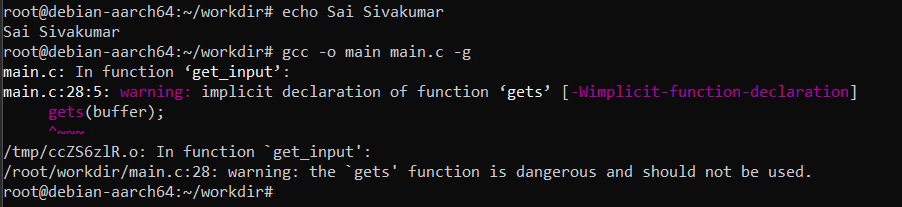
\includegraphics[scale=.85]{compile warning.png}
        \end{center}
    \end{enumerate}
    \item Run \fn{main} from the debugger, without causing buffer overflow. \begin{enumerate}
        \item Addresses of branch and link instructions [Table 1].
        \begin{center}
            \begin{tabular}[h]{|c|c|}
                \hline\textbf{Instruction} & \textbf{Address} \\
                \hline\fn{bl benign\_function} & \fn{0x8c8}\\
                \hline\fn{bl get\_input} & \fn{0x8a4}\\
                \hline
            \end{tabular}
        \end{center}
        \item What are \fn{x29} and \fn{x30}? Why are they placed on the stack?
        
        The registers \fn{x29} and \fn{x30} are the frame pointer and return address, respectively. The frame pointer contains the location of saved registers and local variables for the function called before \fn{main}, and the return address is the address of the line of code the program was at prior to calling \fn{main}. Both need to be pushed and popped off the stack in the right order to ensure correct execution of all functions in any program.
        \item Register values [Table 2].
        \begin{center}
            \begin{tabular}[h]{|c|c|}
                \hline\textbf{Register} & \textbf{Value} \\
                \hline\fn{x29} & \fn{0xfffffffffb00}\\
                \hline\fn{x30} & \fn{0xaaaaaaaaa904}\\
                \hline\fn{SP} & \fn{0xfffffffffaf0}\\
                \hline
            \end{tabular}
        \end{center}
        \item Contents of the stack [Table 3].
        \begin{center}
            \begin{tabular}[h]{|c|c|c|}
                \hline\textbf{Memory Address} & \textbf{Value} & \textbf{Value} \\
                \hline\fn{0xfffffffffaf0} & \fn{0x0000aaaaaaaaa918} & \fn{0x0000000000000000}\\
                \hline\fn{0xfffffffffb00} & \fn{0x0000fffffffffb20} & \fn{0x0000ffffb7ea7364}\\
                \hline
            \end{tabular}
        \end{center}
        \item Figure 2.
        \begin{center}
            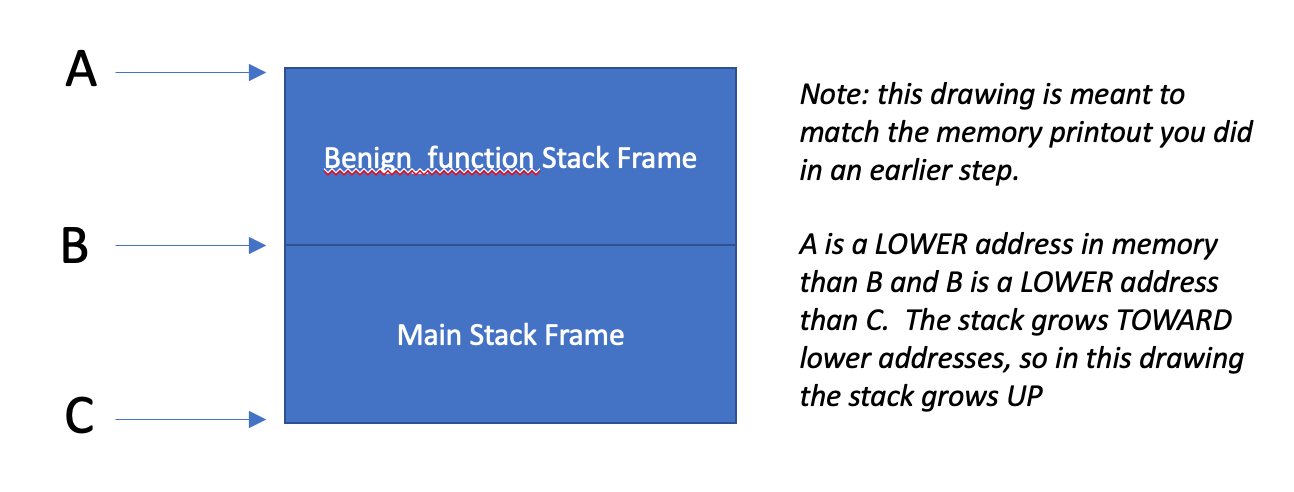
\includegraphics[scale=.55]{figure2.png}
        \end{center}
        \item In Figure $2$, \textbf{A} points to \fn{0xfffffffffaf0} and \textbf{B} points to \fn{0xfffffffffb00}.
        \item The values of \fn{x29} and \fn{x30} written to the stack frame earlier in the execution of \fn{main} was \fn{0x0000fffffffffb20} and \fn{0x0000ffffb7ea7364} respectively.
        \item The address pointed to by \textbf{C} is \fn{0xfffffffffb10}.
        \item Register values [Table 4]. Note that the stack pointer value is smaller.
        \begin{center}
            \begin{tabular}[h]{|c|c|}
                \hline\textbf{Register} & \textbf{Value} \\
                \hline\fn{x29} & \fn{0xfffffffffb00}\\
                \hline\fn{x30} & \fn{0xaaaaaaaaa904}\\
                \hline\fn{SP} & \fn{0xfffffffffb00}\\
                \hline
            \end{tabular}
        \end{center}
        \item Contents of the stack [Table 5]. Highlighted in pink is my input, \fn{saisudha} (and it appears in reverse order, i.e., \fn{s} corresponds to \fn{73}).
        \begin{center}
            \begin{tabular}[h]{|c|c|c|}
                \hline\textbf{Memory Address} & \textbf{Value} & \textbf{Value} \\
                \hline\fn{0xfffffffffae0} & \fn{0x0000fffffffffb00} & \fn{0x0000aaaaaaaaa90c}\\
                \hline\fn{0xfffffffffaf0} & \fn{0x00000007aaaaa918} & \fn{0x}\leftbox{\fn{6168647573696173}}\\
                \hline\fn{0xfffffffffb00} & \fn{0x0000fffffffffb00} & \fn{0x0000ffffb7ea7364}\\
                \hline
            \end{tabular}
        \end{center}
        \item The data in memory shown in the top row is the saved frame pointer (register \fn{x29}) and return address (register \fn{x30}) after stepping into \fn{get\_input} from \fn{main}. The frame pointer points to the stack frame for \fn{main}.
    \end{enumerate}
    \item Run \fn{main.c} from the debugger, causing buffer overflow. \begin{enumerate}
        \item Contents of the stack [Table 6]. Highlighted in pink is my input, \fn{123456789012345678} (and it appears in reverse order, i.e., \fn{1} corresponds to \fn{31}).
        \begin{center}
            \begin{tabular}[h]{|c|c|c|}
                \hline\textbf{Memory Address} & \textbf{Value} & \textbf{Value} \\
                \hline\fn{0xfffffffffae0} & \fn{0x0000fffffffffb00} & \fn{0x0000aaaaaaaaa90c}\\
                \hline\fn{0xfffffffffaf0} & \fn{0x00000007aaaaa918} & \fn{0x}\leftbox{\fn{3837363534333231}}\\
                \hline\fn{0xfffffffffb00} & \fn{0x}\leftbox{\fn{3635343332313039}} & \fn{0x0000ffffb700}\leftbox{\fn{3837}}\\
                \hline
            \end{tabular}
        \end{center}
        \item The stack frame for \fn{main} has changed. Now part of my input has been stored in what should be the frame pointer for the function called before \fn{main}. Specifically the values for the ninth through the sixteenth characters (the second set of eight characters) are stored there, and the remaining two characters' values make it to the stored return address (smiles wickedly \darkhappy). 
        \item Register values [Table 7]. 
        \begin{center}
            \begin{tabular}[h]{|c|c|}
                \hline\textbf{Register} & \textbf{Value} \\
                \hline\fn{x29} & \fn{0x}\leftbox{\fn{3635343332313039}}\\
                \hline\fn{x30} & \fn{0xffffb7003837}\\
                \hline\fn{SP} & \fn{0xfffffffffb20}\\
                \hline
            \end{tabular}
        \end{center}
        \item Indeed, \fn{0x}\leftbox{\fn{3635343332313039}} is loaded onto \fn{x29} and \fn{0x0000ffffb700}\leftbox{\fn{3837}} is loaded onto \fn{x30}, with the highlighted parts being part of my input (cf. comment in (b)).
        \item Stepping forward yields the following error:
        \begin{center}
            \fn{Cannot find bounds of current function}
        \end{center}
        This happens because the contents of \fn{x29} and/or \fn{x30} are corrupted.
    \end{enumerate}
    \item Record address for \fn{arbitrary\_code} function. \begin{enumerate}
        \item The address in memory of the first line of the \fn{arbitrary\_code} function is \fn{0x0000000000000878}.
    \end{enumerate}
    \item Run \fn{main} from command line, overflow the buffer. \begin{enumerate}
        \item Screenshot of running \fn{main} with $20$ character input.
        \begin{center}
            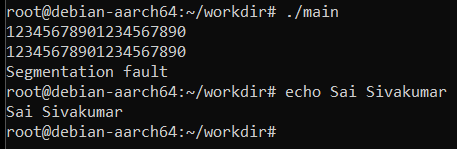
\includegraphics[scale=0.85]{segfault.png}
        \end{center}
        \item The code seems to do what it says it should do, but a segmentation fault occurs.
    \end{enumerate}
    \item Run \fn{main} from command line, craft input to \fn{main} to execute \fn{arbitrary\_code} function. \begin{enumerate}
        \item Address space layout randomization (ASLR) basically randomizes the positions of the stack and of memory addresses a program will use upon execution. ASLR is needed to make buffer overflow attacks more difficult as attackers need to know the location of executables in memory. For us, we turn ASLR off in order to have the memory addresses of the functions remain fixed, so that we can correctly inject the memory address of \fn{arbitrary\_code} into \fn{main}'s stack frame. (\href{https://docs.oracle.com/en/operating-systems/oracle-linux/6/security/ol_aslr_sec.html}{Oracle\textsuperscript{\tiny\textregistered} Linux 6 Security Guide} and \href{https://www.ibm.com/docs/en/zos/3.1.0?topic=overview-address-space-layout-randomization}{IBM z/OS documentation})
        \item Use the command \begin{center}
            \fn{echo -e "1234567812345678\textbackslash x78\textbackslash xa8\textbackslash xaa\textbackslash xaa\textbackslash xaa\textbackslash xaa" | ./main}
        \end{center}
        to cause the code in \fn{arbitrary\_code} to run and loop indefinitely, printing the lines
        \begin{center}
            \fn{Now you know I should not be seen !}\\
            \fn{But I am. Don't believe me just watch}
        \end{center}
        over and over again.
    \end{enumerate}
    \item Turn ASLR back on. \begin{enumerate}
        \item Turning ASLR back on causes \fn{main} to print out part of the input followed by a segmentation fault. It seems the code in \fn{arbitrary\_code} does not execute.
    \end{enumerate}
    \item Fix the vulnerability. \begin{enumerate}
        \item If \fn{gets(buffer)} is replaced by \fn{fgets(buffer, 8, stdin)} in \fn{main.c} and we pass in an input greater than $8$ characters, execution of the new \fn{main} prints out only the first seven characters of the input onto the screen without any errors.
    \end{enumerate}
    \item Find a stack buffer overflow vulnerability on the CVE website. \begin{enumerate}[left = \parindent, label=\href{https://cve.mitre.org/cgi-bin/cvename.cgi?name=CVE-2023-29284}{CVE-2023-29284}:] 
    \item Adobe Substance 3D Painter USDA File Parsing Stack-based Buffer Overflow Remote Code Execution Vulnerability (see [\href{https://cve.mitre.org/cgi-bin/cvename.cgi?name=CVE-2023-29284}{1}], [\href{https://www.cve.org/CVERecord?id=CVE-2023-29284}{2}], [\href{https://helpx.adobe.com/security/products/substance3d_painter/apsb23-29.html}{3}], and [\href{https://cwe.mitre.org/data/definitions/121.html}{4}])
    \end{enumerate}
    The affected software is the Adobe Substance 3D Painter software versions 8.3.0 and earlier.

    It seems Adobe Systems Incorporated themselves submitted the vulnerability to CVE, acknowledging the work of Mat Powell and Trend Micro Zero Day Initiative.

    The vulnerability is CWE-121: Stack-based Buffer Overflow, which is when a buffer being overwritten is allocated on the stack (e.g. a local variable) and leads to things like return addresses being overwritten (like in this lab). For this vulnerability, it would have been possible for the Adobe software to execute arbitrary code, but to exploit this vulnerability, a victim must have malicious files open.

    I think vulnerabilities like these still occur since there may be procedures which freely read input and write to memory, and programmers forget to check against the expected length or type of input. Providing incorrect inputs could cause incorrect execution of these procedures which overwrite items allocated on the stack (like return addresses).
\end{enumerate}
\end{document}